\documentclass{beamer}
\usepackage{graphicx}
\usepackage{paralist}
\usepackage{outlines}

\title{Marquee Tools}
\author{Mendocino College - Image Manipulation with Photoshop}
\titlegraphic{\vspace{-10mm}
\includegraphics[width = .8\textwidth]{images/photoshop.jpg}} 
\date{\vspace{-5em}} 


\mode <presentation>
\usetheme{Warsaw}
\usecolortheme{default}

\setbeamerfont{footline}{size=\fontsize{5}{8}\selectfont}

\definecolor{darkred}{rgb}{20,0,0}
\definecolor{darkgreen}{RGB}{40,110,20}
\definecolor{darkpurple}{RGB}{30,0,30}
\definecolor{chardonnay}{RGB}{255, 255, 204}

\setbeamercolor*{palette primary}{fg=white, bg=darkgreen}


\begin{document}
	{
		\setbeamertemplate{footline}{} 
		\setbeamertemplate{headline}{} 
		\begin{frame}
			\vspace{-35pt}
			\maketitle
		\end{frame}
	}

	\section{Marquee Tool}
		\begin{frame}
		\frametitle{Marquee Tool}
		\begin{center}
			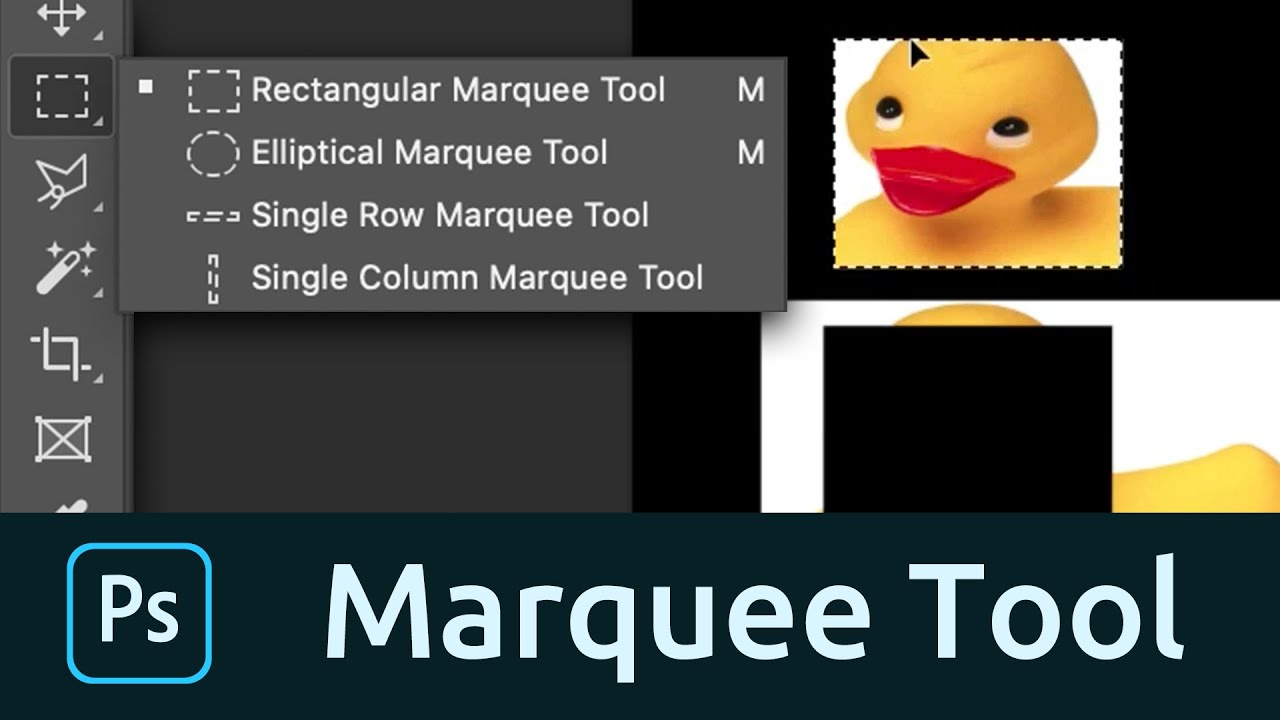
\includegraphics[width = 1.0\textwidth]{images/maxresdefault (3).jpg}
		\end{center}
	\end{frame}
	
			\subsection{What are the Marquee Tools?}		
	\begin{frame}
		\frametitle{What are the Marquee Tools?}
	\begin{outline}
		\1 The marquee tools let you select rectangles, ellipses, and 1‑pixel rows and columns.
		\1 It is one of the basic and most commonly used selection tools in Photoshop. In this article, we will discuss the marquee tool along with its properties and use.
		\1 Marquee tool is the basic selection tool that can select your Photoshop layer in several shapes, like rectangle, ellipse, single-pixel vertical and horizontal line, square, ovals and circles, etc
	\end{outline}
\begin{center}
	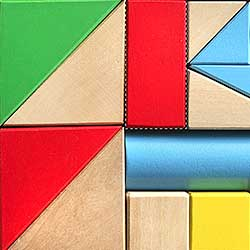
\includegraphics[width=.5\textwidth]{images/photoshop-rectangular-marquee-tool-f.jpg}
	\end{center}
		\end{frame}


\section{Rectangular Marquee Tool}
\subsection{Rectangular Marquee Tool}	
\begin{frame}
	\frametitle{Rectangular Marquee Tool}
	\begin{outline}
		\1 Makes a rectangular selection 
		\1 Hold down the Shift key to make a Square Selection.
		\1 Hold Alt to drag a marquee from its center.

	\end{outline}
	\begin{center}
		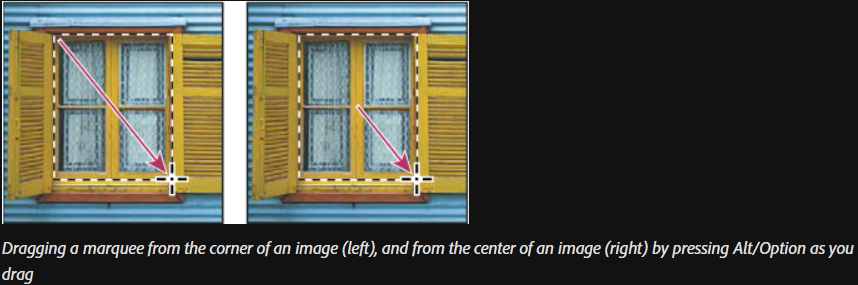
\includegraphics[width = 1.0\textwidth]{images/drag marquee.png}
	\end{center}
\end{frame}

\section{Elliptical Marquee Tool}
\subsection{Elliptical Marquee Tool}	
\begin{frame}
	\frametitle{Elliptical Marquee Tool}
	\begin{outline}
		\1 Makes a elliptical selection 
		\1 Hold down the Shift key to make a Circle Selection.
		\1 Normal
		\2 Determines marquee proportions by dragging.
		\1 Fixed Ratio
		\2 Sets a height-to-width ratio. Enter values (decimal values are valid) for the aspect ratio. 
		\3 For example, to draw a marquee twice as wide as it is high, enter 2 for the width and 1 for the height.
		\1 Fixed Size
		\2 Specifies set values for the marquee’s height and width. 
		\3 Enter pixel values in whole numbers.
	\end{outline}
	\begin{center}
		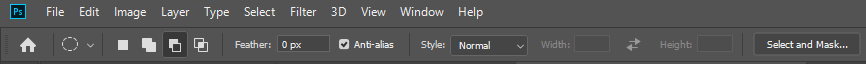
\includegraphics[width = 1.0\textwidth]{images/elliptical marquee.png}
	\end{center}
\end{frame}

	
\section{Single Row or Single Column Marquee Tool}
\subsection{Single Row or Single Column Marquee Tool}	
\begin{frame}
	\frametitle{Single Row or Single Column Marquee Tool}
	\begin{outline}
		\1 Defines the border as a 1‑pixel‑wide row or column.
		\1 Click near the area you want to select, and then drag the marquee to the exact location. 
		\2 If no marquee is visible, increase the magnification of your image view.
	\end{outline}

\end{frame}


\end{document}